\chapter{CMS detector and LHC}
This thesis is done via analyzing the data collected by the Compact Muon Solenid (CMS) detector at the Large Hadron Collider (LHC). CMS is one of the two largest detectors built on the LHC. This chapter will briefly introduce the LHC and the CMS detector.

\section{Large Hadron Collider}
The LHC is the world's most powerful hadron collider and the largest experimental facility ever. It was built by the European Organization for Nuclear Research (CERN) between 1998 and 2008 in collaboration with over 10,000 scientists and engineers from over 100 countries, as well as hundreds of universities and laboratories. It lies in a tunnel 27 km in circumference, as deep as 175 m beneath the France$-$Switzerland border near Geneva. The designed maximum collison energy and highest luminosity of the LHC are 14 TeV and $\textup{10}^{-34} \textup{cm}^{-2}\textup{s}^{-1}$ respectively.

Other accelerators that had been originally built at CERN for previous experiments is working as an injection chain for the LHC now. The proton beam starts from LINAC, a small linear accelerator, where its energy firstly reaches 50 MeV. It then passes through a booster and goes to the PS, where it is accelerated up to 25 GeV. After that, it reaches 450 GeV in the SPS. The beam is finally injected in the LHC ring from the SPS, it is accelerated up to 4 TeV in 2012. In early 2015, the proton beam had been acceletated to 6.5 TeV, a value near its designed energy, before undergoing collision.

There are four collision points at the LHC, corresponding to four main experiments, CMS, ATLAS, LHCb and ALICE. The ALICE experiment is optimized to study heavy-ion (Pb-Pb nuclei) collisions and focusing on the physics of strongly interacting matter at extreme energy densities. LHCb is a specialized b-physics experiment, measuring the parameters of CP violation in the interactions of b-hadrons. Such studies can help to explain the matter-antimatter asymmetry of the universe. Last, CMS and ATLAS are two general purpose detectors. The aims of these two experiments are investigating a wide range of physics, including the search for the beyond standard model particles, extra dimensions, and dark matter.


\begin{figure}[hbtp]
  \begin{center}
    \includegraphics[width=0.9\textwidth]{figure/CH2/CERN_Overview.jpg}
  \end{center}
  \caption{\label{fig:LHC_overview}Overview of the LHC and relative location of the detectors.}
\end{figure}

\begin{figure}[hbtp]
  \begin{center}
    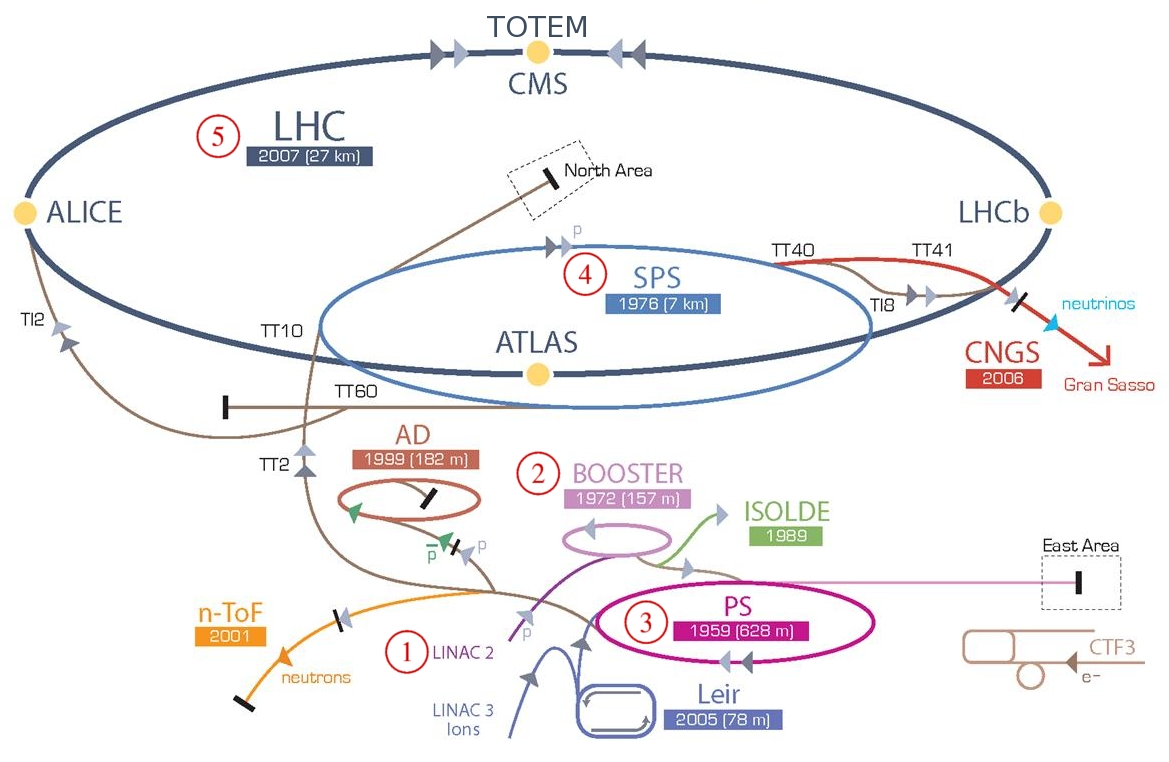
\includegraphics[width=0.9\textwidth]{figure/CH2/complex.png}
  \end{center}
  \caption{\label{fig:accelerator}CERN accelerator complex.}
\end{figure}

\section{Compact Muon Solenoid}
The Compact Muon Solenoid (CMS) detector is designed to cope very high rate of interactions expected to take place at the high LHC luminosity. It has the typical structure of detectors at hadron colliders: a central region ($barrel$) enclosed by two disks ($endcaps$). The structure of CMS can be seen in Fig.~(\ref{fig:CMS}).

\subsection*{Solenoid and Sub-detectors}
CMS features a powerful superconducting coil, generating a solenoidal magnetic field around 3.8 Tesla in a large volume, which hosts different sub-detctors. The magnetic field lines close through steel yoke in the outer region and the distinct sub-detectors are designed in order to obtain the highest possible resolution and the largest acceptance for every kind of particles.

The innermost layer is a silicon-based tracker. Surrounding it is a scintillating crystal electromagnetic calorimeter (ECAL), which is itself surrounded with a sampling calorimeter for hadrons (HCAL). The tracker and the calorimeters are compact enough to fit inside the CMS Solenoid. Outside the magnet are the large muon detectors separated by layers of the steel yoke.

\begin{figure}[hbtp]
  \begin{center}
    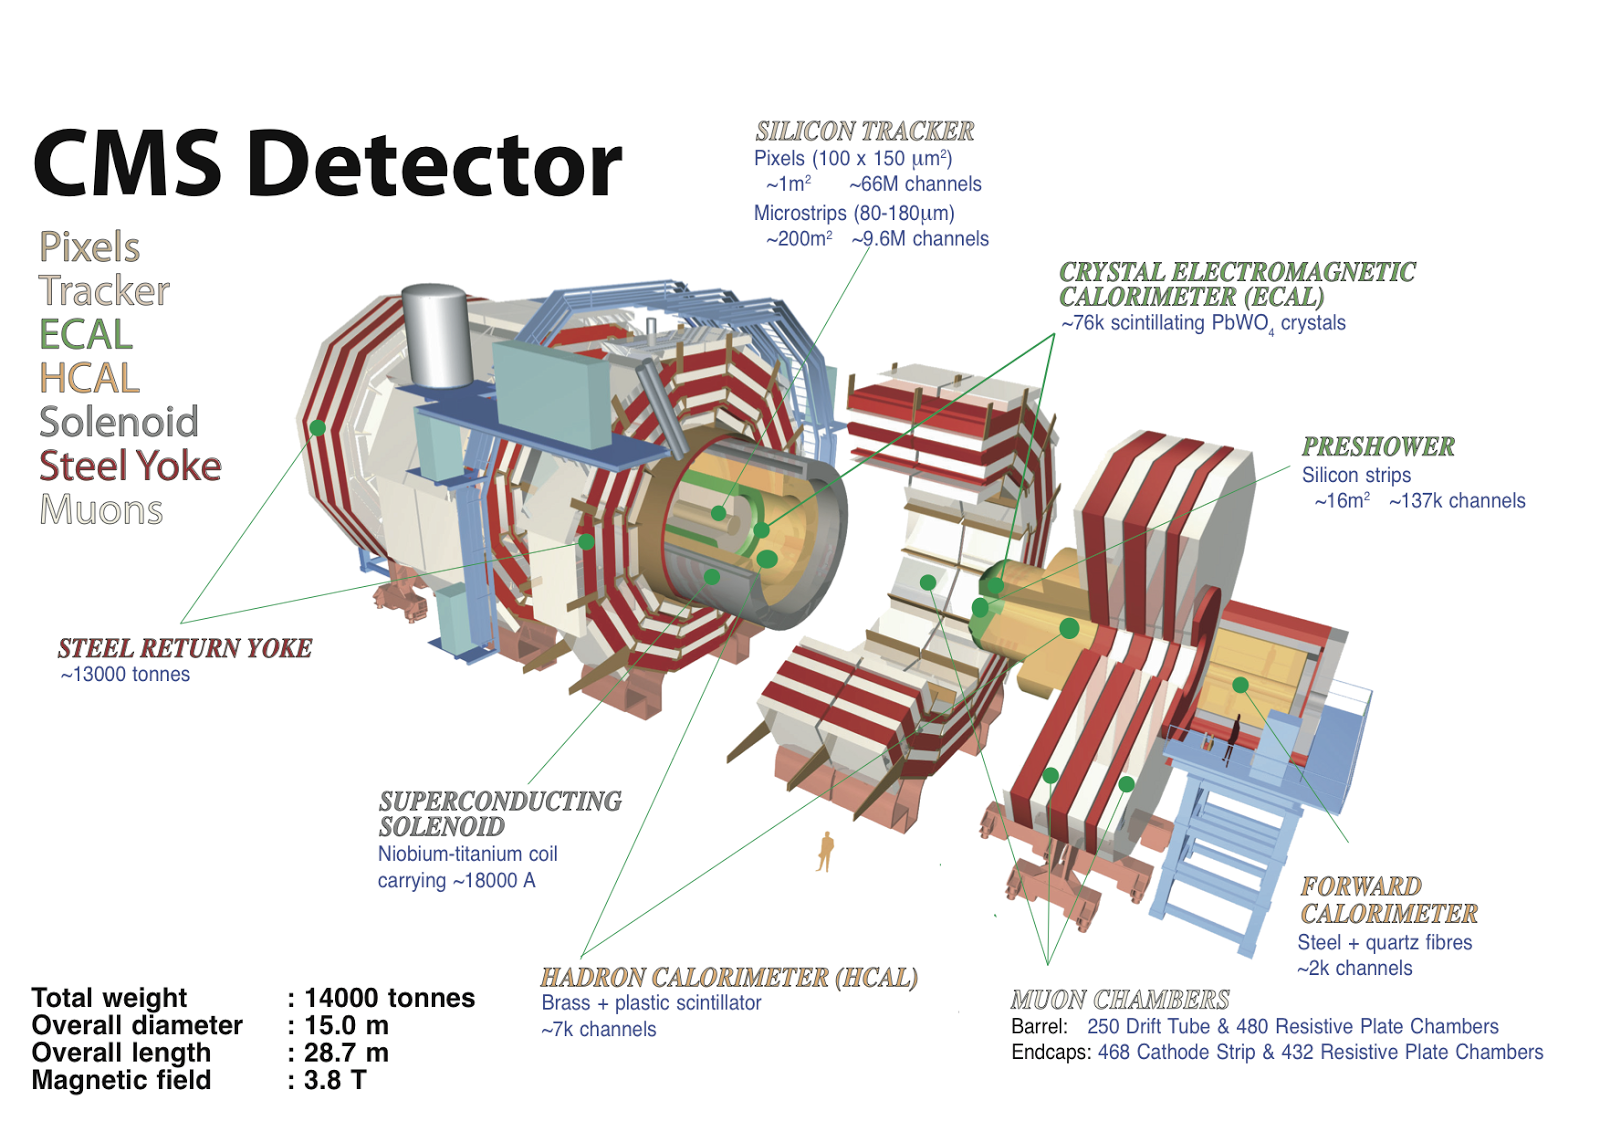
\includegraphics[width=0.9\textwidth]{figure/CH2/CMS.png}
  \end{center}
  \caption{\label{fig:CMS}Structure overview of the CMS detector.}
\end{figure}
\subsection*{Coordinate System}

The CMS coordinate system is oriented such that the $x$-axis points to the center of the LHC ring, the $y$-axis points vertically upward and the $z$-axis is in the direction of the beam. The azimuthal angle $\phi$ is measured from the $x$-axis in the $xy$ plane and the radial coordinate in this plane is denoted by $r$. The polar angle $\theta$ is defined in the $rz$ plane, while the pseudo-rapidity $\eta=-ln\tan{(\theta/2)}$. The momentum component transverse to the beam direction, denoted by $p_{T}$, is computed from the $x$- and $y$-components, and the transverse energy is defined as $E_{T}=E\sin\theta$.

\subsection{Tracker}
Tracker is the most inner part of CMS that contacts the productions of collisions in the first place. It traces the charged particles' trajectories without considering their energy as possible. Physicists can reconstruct the vertices of the interaction and the momentum of charged particles by linking tracks to the collider's pipe and measuring the curves of particles under magnetic field.

The tracking system is composed of two kinds of detector, the pixel detector and silicon strip detector. The pixel detector is built from three barrel layers at $r$=44, 73, 102 mm, and two endcap disks on each side at $z$=$\pm$345, $\pm$465 mm.
\begin{figure}[hbtp]
  \begin{center}
    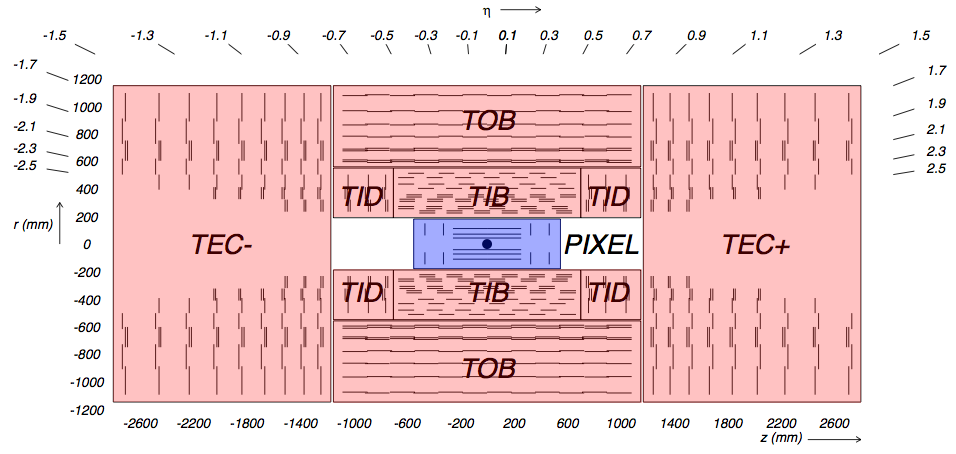
\includegraphics[width=0.9\textwidth]{figure/CH2/tracker.png}
  \end{center}
  \caption{\label{fig:tracker}Schematic layout of tracker.}
\end{figure}
\begin{figure}[hbtp]
  \begin{center}
    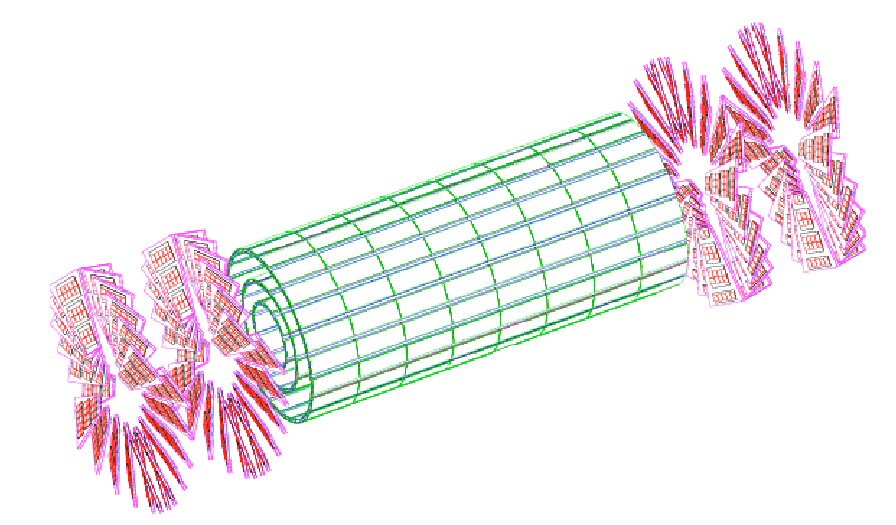
\includegraphics[width=0.4\textwidth]{figure/CH2/pixel.png}
  \end{center}
  \caption{\label{fig:pixel}The pixel detector inside tracker.}
\end{figure}
\newline And the pixel detector consists of 1440 segmented silicon sensor modules with total 66 millon readout channels. Charge carriers are distributed over several pixels. The analog pulse height information can be used to calculate the center of certain charge distribution which could improve the hit information. The spatial resolution is measured to be about 10 $\mu m$ for the $r-\phi$ plane or about 20 $\mu m$ for $z$ direction measurement.

Outside the pixel detector, there comes the silicon strip detector. The barrel region of silicon strip detector is divided into two parts, the Tracker Inner Barrel (TIB) and the Tracker Outer Barrel (TOB). The former is composed of four layers of silicon sensors with a thickness of 320 $\mu m$ and of strip pitches varying from 80 to 120 $\mu m$. The TOB is made of six layers. In this sub-detector thicker silicon sensors (500 $\mu m$) are employed, while the strip pitch varies from 120 to 180 $\mu m$. The endcap region ($|\eta| >$ 1.6) is covered by the Tracker Inner Disks (TID) and the Tracker End Cap (TEC). The entire silicon strip detector is comprised of 15200 high-sensitivity modules consisting of detecting unit, supporting structure and readout electonic system.

\subsection{ECAL}

The Electromagnetic Calorimeter (ECAL) measures the energy of photons, electrons and positrons. It it is placed just outside the tracker, but still inside the solenoid. ECAL is made of 74848 lead-tungstate (PbWO$_{4}$) crystals. This material is characterized by a high density (8.28 g/cm$^3$ ), which gives the crystals a very compact form and makes them particularly suitable to be placed inside the magnetic coil. Another reason, this material has also a fast temporal response ($\sim$10 ns) and its radiation length (X$_{0}$) of 0.89 cm give ECAL the possibility to fully contain the expansion of the electromagnetic shower.

The arrangement of ECAL is shown in Fig.~(\ref{fig:ECAL}). The barrel crystals have a front face area of 2.2 $\times$ 2.2 cm$^2$ and a length of 23 cm. They are positioned at $r$= 1.29 m in pseudo-rapidity region 0 $< |\eta| <$ 1.479. The crystals in the endcaps have a 2.47 $\times$ 2.47 cm$^2$ front face, a 22 cm length and they are positioned at $z$= 3.17 m in 1.479 $< |\eta| <$ 3.0. A Preshower detector is placed in front of the endcaps crystals. The active elements of Preshower are two planes of silicon strips with a pitch of 1.9 mm, which lie behind disks of lead absorber at depths of 2X$_{0}$ and 3X$_{0}$. It allows the rejection of photon pairs from $\pi^{0}$ decays and improvesthe estimation of the direction of photons, to enhance the measurement of the two-photon invariant mass.

The energy resolution of the ECAL is given by three different contributions\cite{EcalReso},
\begin{align}
\frac{\sigma_{E}}{E}=\frac{a}{\sqrt{E}}\oplus\frac{b}{E}\oplus c
\end{align}
where the first term is statistical in nature, it also contains fluctuation in showering and in the amplification through photodiodes (a$\sim$2.8\%), the second one considers electronic noise and pile-up (b$\sim$12\%) and the last term is mainly due to the calibration (c$\sim$0.3\%).

\begin{figure}[hbtp]
  \begin{center}
    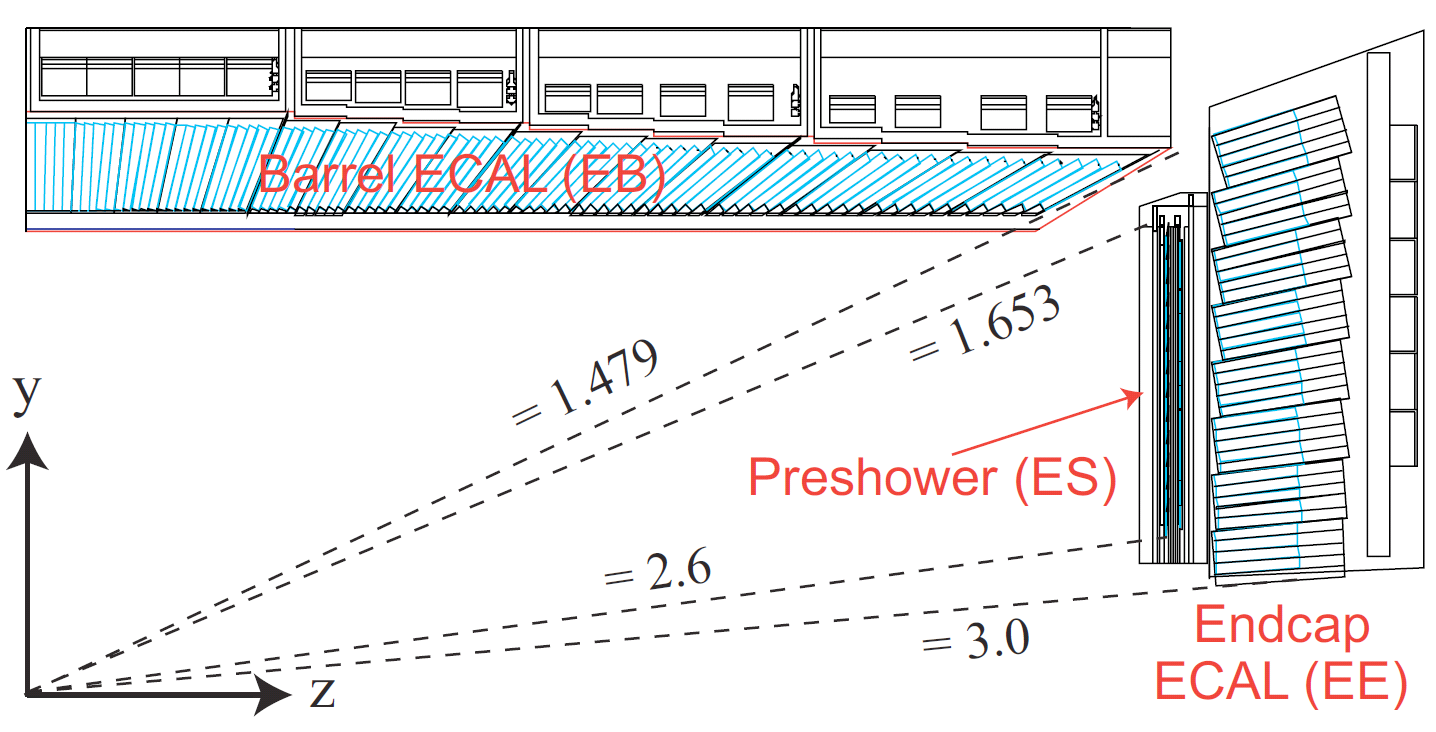
\includegraphics[width=0.9\textwidth]{figure/CH2/ECAL.png}
  \end{center}
  \caption{\label{fig:ECAL}Schematic layout of the CMS ECAL.}
\end{figure}










\subsection{HCAL}
\subsection{Muon Chamber}
\subsection{Trigger System}
